\subsection{the Continuous Opioid Spread Model}
Our model is inspired by the Porous Media Contaminant Transport Model.\cite{8} The transport process is expressed by a differential equation, balancing the total mass of contaminant in the fracture. 

Similarly, we propose a Continuous Opioid Spread(COS) model. This model, which is expressed through a partial differential equation, views the geographical and time attributes in a continuous way. 

Let $S(x,y,t)$ be the amount of opioid stored in $(x,y)$ at time $t$, and $U(x,y,t)$ the amount of opioid used or consumed by population in $(x,y)$ at time $t$.
\begin{comment}
, and $F(x,y,t)$ as the amount of drugs identified in $(x,y)$ at time $t$. We assume that the amount of identified drugs is directly proportional to the total amount of drugs with a proportionality constant $k$, such that

The NFLIS data contains opioid identification counts in years 2010-2017 for narcotic analgesics and heroin in each of the counties from the five states stated in the problem background section. We denote this data as $F(x,y,t)$, the amount of drugs identified in $(x,y)$ at time $t$. 

\begin{equation}
S(x,y,t) = k F(x,y,t)
\end{equation}
\end{comment}
Since the amount of opioid used is less than or equal to the amount of opioid stored in the same location at the same time, we assume that
\begin{equation}
U(x,y,t) = \lambda S(x,y,t), 0\leq \lambda \leq 1
\end{equation}

where $\lambda$ is an attribute implying the ratio between the amount of opioid use and that of opioid storage. We temporarily overlook the relevance between $\lambda$ and location $(x,y)$.

%It is natural to assume that $\lambda$ is revelant with socio-economical factors of the given location. We shall address this when coping with the second part of the problem.

We use the laplacian operator $\frac{\partial^2 S}{\partial x^2} + \frac{\partial^2 S}{\partial y^2}$ to describe the tendency of opioid spread. Multiplied with a transportation coefficient $D$, it indicates the net opioid amount transported into $(x,y)$ at time $t$.

%We use $D(\frac{\partial^2 S}{\partial x^2} + \frac{\partial^2 S}{\partial y^2})$ to describe the total amount of opioid transported into the city.  describes the tendency of opioid spread, i.e. the trend of transporting opioid from $(x,y)$ to neighboring coordinates.

As a result, in a specific location $(x,y)$, the difference between the net opioid amount transported into $(x,y)$ and the amount of opioid used equals to the change in storage:
\begin{equation}
D(\frac{\partial^2 S}{\partial x^2} + \frac{\partial^2 S}{\partial y^2}) - \lambda S = \frac{\partial S}{\partial t} 
\end{equation}
\begin{comment}
$S$, however, is unknown. We substitute (1) into (3), and eliminate the common factor $k$ from both sides of the equation
\begin{equation}
D(\frac{\partial^2 F}{\partial x^2} + \frac{\partial^2 F}{\partial y^2}) - \lambda F = \frac{\partial F}{\partial t}
\end{equation}
\end{comment}

\subsection{The Discrete Opioid Spread Model}
Based on the continuous model constructed above, we propose an analogous Discrete Opioid Spread Model, which could be directly applied to reality. In such a discrete model, we divide the transporation into two parts: opioid transport-in and transport-out, so that we have two different storage status. $S(t)$ indicates the status after transport-in, but before transport-out, while $S'(t)$ describes the status after transport-out, but before the next transport-in.

\subsubsection{Graph Construction}
In this scenario, we view counties as separate nodes in an \textbf{directed graph}. The edges of the network are determined by the geographical adjacency features. Our data concerning geographically adjacent counties are extracted from the United States Census Bureau\cite{13}. To be precise, node $i$ has an edge pointing towards $j$ when county $i$ and $j$ are neighboring counties. Let $N_i$ be the set of node $i$'s neighboring nodes. Let $v_{ij}(t)$ be the amount of opioid transported from $i$ to $j$ at time $t$. In this way, we construct an directed graph of all counties. 

\subsubsection{Conversion From Continuous Model to Discrete Model}
Now we discuss how to extend the Continuous Opioid Spread Model to this graph. For county $i$ at time $t$, we convert equation (1) into

\begin{equation}
U_i(t) = \lambda\cdot S_i(t), 0\leq \lambda \leq 1 \\
\end{equation}

Next, we attempt to convert (2) to discrete scenarios as well. The $S_{xx}+S_{yy}$ part is an laplacian operator. It demonstrates the difference in opioid amount between two neighboring counties.  Let $T^{IN}_i(t)$ be the total amount of opioid transported into or produced by county $i$ and $T^{OUT}_i(t)$ be the total amount of opioid transported to adjacent counties, so we have

\begin{equation}
T^{IN}_i(t)-T^{OUT}_i(t) - U_i(t)= S'_i(t)-S'_i(t-1)
\end{equation}
and 
\begin{equation}
S_i(t) = T^{IN}_i(t) + S_i'(t-1)
\end{equation}

Combining (4) and (5), the Discrete Opioid Spread Model can be described as
\begin{equation}
T^{IN}_i(t) + S'_i(t-1)-S'_i(t) = \lambda(T^{IN}_i(t) + S'(t-1))+ T^{OUT}_i(t)
\end{equation}
or 
\begin{equation}
(1-\lambda)S_i(t)-S'_i(t) = T^{OUT}_i(t)
\end{equation}

\begin{comment}
\textit{
In the previous subsection, we pointed out that $\lambda$ is a socio-economic factor impling the relationship between opioid usage and opioid storage. In the discrete scenario, we can describe it as
}
\begin{equation}
\lambda = \frac{U_i(t)}{S_i(t)} = \frac{S_i(t) -\sum_{j\in N_i}S_j(t)}{S_i(t)}
\end{equation}
\end{comment}
\subsubsection{Taking A Deeper Look at Opioid Transportation}
Naturally, the question arises on how drugs transported outside a county should be distributed to adjacent counties. We have

\begin{equation}
T^{OUT}_i(t) = \sum_{j\in N_i}v_{ij}(t)
\end{equation}

The laplacian operator is an implication for us to distribute $T^{OUT}_i(t)$ in proportion to the difference in storage between $i$ and its adjacent nodes $j \in N_i$. Thus
%Since $S$ is proportional to $F$ with constant $k$, we can compute the distribution pattern by calculating the difference in the amount of identified drugs $F$
\begin{equation}
v_{ij}(t) = T^{OUT}_i(t)\cdot \frac{S_i - S_j}{\sum_{k \in N_i}(S_i - S_k)}
\end{equation}



\subsection{Identifing the Origin of Specific Opioid Use}
We compose a 3D image illustrating the characteristics of the specific opioid (e.g. heroin) cases across counties. We transform the FIPS coding of the counties into their latitude and longitude based on data from the U.S. Census Bureau\cite{14}. The x-axis represents the latitude, the y-axis represents the longitude, and the z-axis represents the amount of specific opioid reports, which we denote as $F(x,y)$.(Figure 1(a))

\textit{NOTE: The opioid report amount $F$ is has a strong connection with opioid storage $S$. According to equation (3), we can infer that opioid usage $U$ is also connected with $F$. Therefore, under valid circumstances we shall use the known data $F$ to reflect the unknown data $S$ or $U$ hereafter.}

We construct a continuous 3D model of the latitude-longitude-drugreport relationship using Delaunay Triangulation Method for interpolation, which transforms the scattered point data into a data grid. According to our assumption($\mathcal{A}1-2$), a Source of a specific opioid use should reach a local maximum in opioid reports. An Origin, which is a subset of Sources, possesses almost the same statistical features. A contour map(Figure 1(b)) may help us visualize this ideology.

\begin{figure}[H]
	\centering
	\subfigure[3D Plot]{
		\centering
		\begin{minipage}[t]{0.3\linewidth}
			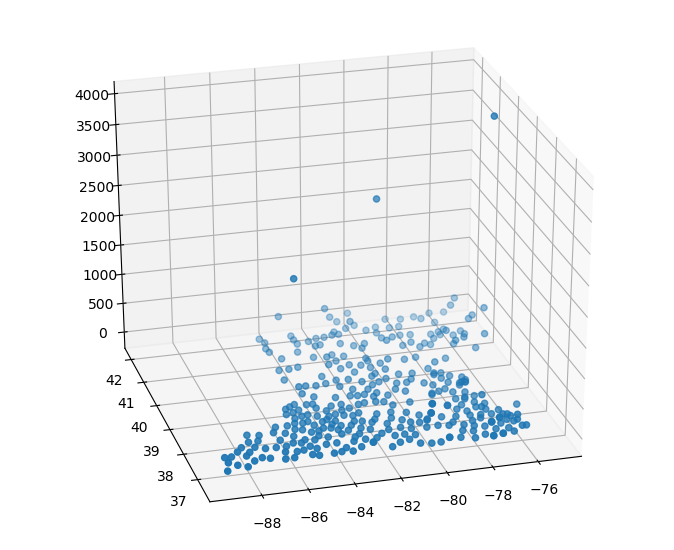
\includegraphics[width=2in]{003}
		\end{minipage}	
	}
	\subfigure[Contour Map]{
		\centering
		\begin{minipage}[t]{0.4\linewidth}
			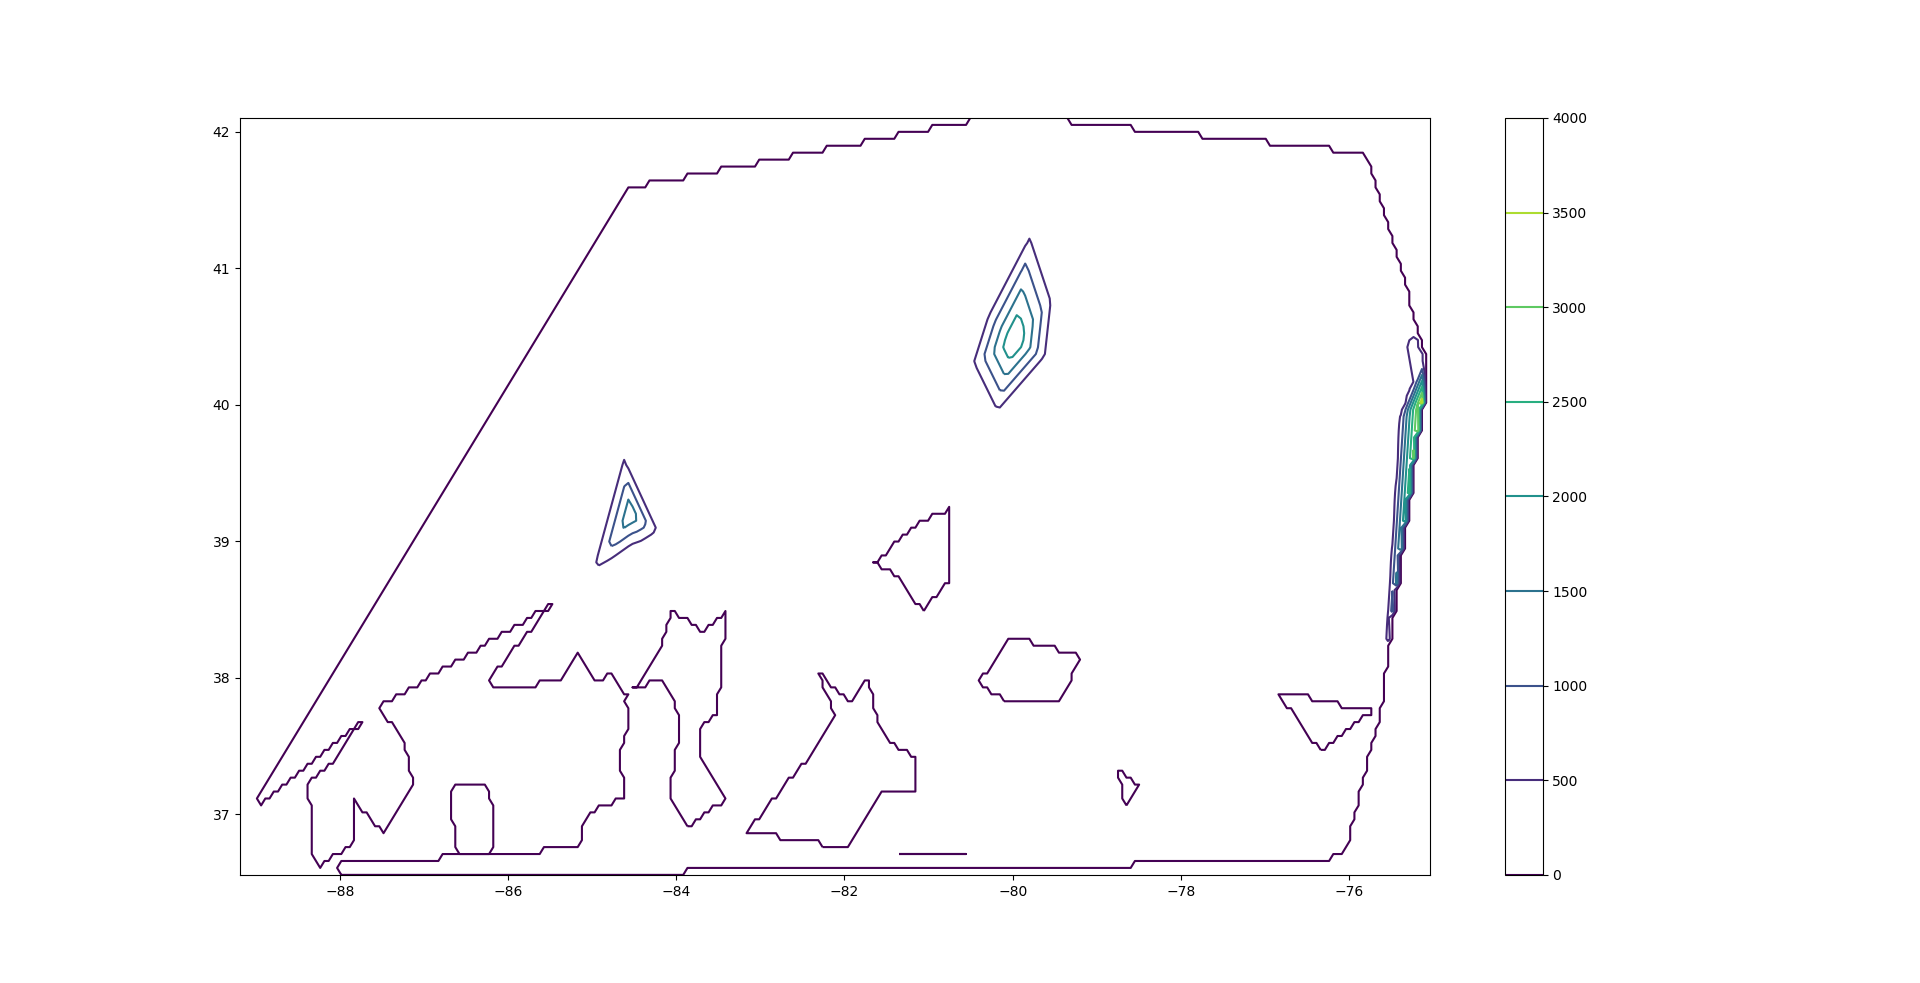
\includegraphics[width=3in]{002}
		\end{minipage}
	}
	\caption{Heroin Data in Year 2010}
\end{figure}

The dataset only consists of data ranging from 2010 to 2016, which is far too limited for us to simulate or infer the actual Origin. Therefore, we can only detect \textbf{\itshape Possible Origins} by examining local maxima.

As we indicated in assumption $\mathcal{A}3$, not all Sources are Origins, and thus not all local maxima are Origins. We need to set up a threshold to distinguish Sources from Origins. 

Therefore, we identify the possible locations where specific opioid use might have started by computing all local maxima(see algorithm 1), and rank them to find the Possible origins in each of the five states. 

\IncMargin{1em}
\LinesNumbered
\begin{algorithm}[H]
	\SetKwData{Left}{left}\SetKwData{This}{this}\SetKwData{Up}{up}
	\SetKwFunction{Union}{Union}\SetKwFunction{FindCompress}{FindCompress}
	\SetKwInOut{Input}{input}\SetKwInOut{Output}{output}
	
	\KwData{2-dimensional array denoting the opioid reports in all counties}
	\KwResult{local maximum index list}	
	\BlankLine
	initiaize local maximum index list to []
	initialize x=0, y=0\;
	\While{not at the end of the array}{
		apply $3\times 3$ maximum filter to the array at position $(x,y)$ \;
		increment $(x,y)$ \;
	}
	initialize x=0, y=0\;
	\While{not at the end of the array}{
		compare the filtered array with the original one at position$(x,y)$ \;
		\If{equal}{
			push $(x,y)$ into the local maximum index list\;
		}
		increment $(x,y)$\;
	}
	\caption{Searching for Local Maxima}
\end{algorithm}
\DecMargin{1em}

The details of our ranking scheme concerns a comparison of a certain county's data in time. A Source has to satisfy the requirement that it reaches local maximum and is greater than a certain threshold. Here for specific opioids, we use its average drug reports as a threshold. 

If a county remains a Source more than 4 years among 2010-2017, then we define it as a \textbf{\itshape Candidate} for the Possible Origin of that state. For each state, if the number of Candidates is greater than 3, then we select the counties ranking top three in specific opioid reports as the Possible Origin for that state. Otherwise, all Candidates are chosen as Possible Origins.

For heroin, the average drug reports is 92. Therefore, using 92 as a threshold and  after conducting the above operations on our dataset, we discovered the following Possible Origins:

\begin{table}[H]
	\centering
	\begin{tabular}{|c|c|c||c|c|c|}
		\hline
		\rowcolor[HTML]{656565} 
		{\color[HTML]{FFFFFF} \textbf{STATE}} & {\color[HTML]{FFFFFF} \textbf{COUNTY}} & {\color[HTML]{FFFFFF} \textbf{F}} &{\color[HTML]{FFFFFF} \textbf{STATE}} & {\color[HTML]{FFFFFF} \textbf{COUNTY}} & {\color[HTML]{FFFFFF} \textbf{F}}\\ \hline
		KY & - & - &WV & Berkeley & 111 \\ \hline
		VA & Richmond City & 237 &WV & Kanawha & 2175\\ \hline
		VA & Prince William & 176 & WV& Harrison&110 \\ \hline
		OH & Hamilton & 3076 &PA & Philadelphia & 3905 \\ \hline
		OH & Cuyahoga & 915 & PA & Allegheny & 2970 \\ \hline
		OH & Lake & 441 & PA & Luzerne & 579\\ \hline
	\end{tabular}
	\centering
	\caption{Possible Origins of Heroin for Each State}
\end{table}

\subsection{General Opioid Identification Threshold}
We endeavor to propose a opioid identification threshold such that when a county's total opioid report reaches this threshold, the U.S. government should be extremely concerned with opioid control in this county.

In order to predict the use/trend-in-use of opioids, it is impossible to predict basing on specific drugs in that the data would be too volatile to conduct a valid prediction. In this context, we choose the total opioid report to conduct a prediction.

\begin{table}[H]
\centering
\begin{tabular}{|c|c|c|}
\hline
\rowcolor[HTML]{656565} 
{\color[HTML]{FFFFFF} \textbf{YEAR}} & {\color[HTML]{FFFFFF} \textbf{AVERAGE}} & {\color[HTML]{FFFFFF} \textbf{TOP 5\%}} \\ \hline
2010 & 540.18 & 1967 \\ \hline
2011 & 525.23 & 1849 \\ \hline
2012 & 540.52 & 1678 \\ \hline
2013 & 557.51 & 1919 \\ \hline
2014 & 556.40 & 1689 \\ \hline
2015 & 573.81 & 1999 \\ \hline
2016 & 579.01 & 1994 \\ \hline
2017 & 600.01 & 2004 \\ \hline
\end{tabular}
\centering
\caption{The Average Opioid Cases per County v.s. The Top 5\% Opioid Cases across Counties from 2010-2017}
\end{table}

Statistics from the dataset reveal that on average, 600 cases of opioid identifications occur in a county per year. Traversing the map, we find that in counties with severe opioid crisis, thousands of opioid identification may occur per year. Under this premesis, we extend the definition of threshold in the previous section and classify the Sources into three levels(see Table 2).


\begin{table}[H]
	\centering
	\begin{tabular}{|c|c|}
		\hline
		\rowcolor[HTML]{656565} 
		{\color[HTML]{FFFFFF} \textbf{Level}} & {\color[HTML]{FFFFFF} \textbf{Threshold}} \\ \hline
		First-level Source  & total Opioid Report per year $\geq 2000$ \\ \hline
		Second-level Source & $600 \leq$ total Opioid Report per year $\leq 2000$ \\ \hline
		Third-level Source  & total Opioid Report per year $\leq 600$ \\ \hline
	\end{tabular}
	\caption{Thresholds}
\end{table}

These three levels indicate the degree at which the U.S. government need to be alarmed. First-level Sources are counties suffering from severe opioid crisis. Second-level Sources have a great potential of becoming first-level Sources. We neglect the discussion of third-level Sources due to limited government management resources.

The strategy against different level of origins varies. First-level Sources require immediate and intense control and intervention, while third-level origins could be treated with milder approaches like propoganda against Opioid misuse. 

The government should also be extremely alarmed about a second-level Source county which has a high likelihood of becoming a first-level Source. We identify them by filtering out all counties which was a Source for over four times in the last eight years, and that the average total opioid report in the last eight years exceeds 600.


\subsection{Model Prediction via the Grey Method}
The database provides us with the record of total opioid identification cases from 2010 to 2017. We hope to predict which counties are in danger of becoming first-level Sources and when. We could use Grey Method to predict the future data based on our current model.

The Gray Model is applied mainly on incomplete data and undeterminable problems. We the use GM(1,1) model for prediction.\cite{12}

Let $X$ be a sequence of observed data, such that
\begin{equation}
X^{(0)} = (X^{(0)}(1),X^{(0)}(2),\cdots,X^{(0)}(n))
\end{equation}
Here, $X^{(0)}(i)$ represents the observed data at time $i$. We generate the first-order Accumulated Generating Operation sequence  $X^{(1)}(i)$ based on $X^{(0)}(i)$, where
\begin{equation}
X^{(1)}(i) = \sum_{k=1}^i X^{(0)}(k) = X^{(1)}(i-1)+X^{(0)}(i)
\end{equation}
Then we establish the first-order differential equation of $X^{(1)}(i)$ as
\begin{equation}
\frac{dX^{(1)}}{dt}+aX^{(1)}=u
\end{equation}
where $a$ and $u$ are parameters we wish to obtain. (6) and (7) reveal that
\begin{equation}
\hat{X}^{(1)}(i+1) = (X^{(0)}(1)-\frac{u}{a})e^{-ai}+\frac{u}{a}
\end{equation}
Now we attempt to fit parameter $a$ and $u$, as described in (7). Let $\hat{a}$ be a sequence of parameters where $\hat{a}=[a,u]^T$. The solution to $\hat{a}$ is
\begin{equation}
\hat{a} = (B^T B)^{-1}B^TY_n
\end{equation}
where
\begin{equation}
B=\left[
\begin{array}{cc}
-\frac{1}{2}[X^{(1)}(1)+X^{(1)}(2)] & 1\\
-\frac{1}{2}[X^{(1)}(2)+X^{(1)}(2)] & 1\\
\cdots & \cdots \\
-\frac{1}{2}[X^{(1)}(n-1)+X^{(1)}(n)] & 1\\
\end{array}
\right],
Y_n = [X^{(0)}(2),X^{(0)}(3),\cdots, X^{(0)}(n)]^T
\end{equation}

Applying GM(1,1) prediction to our data, we find that there are four different types of time-scale data:
\begin{enumerate}
	\item There is no obvious growing trend in time, and therefore impossible to use GM(1,1) to predict when total opioid reports shall reach 2000. In Table 4, the data showed no obvious increase or decrease, but fluctuates with a low variance. It is impossible to predict when will this county become first-level Source.
	\begin{table}[H]
		\centering
		\begin{tabular}{|c|c|c|c|c|c|c|c|}
			\hline
			\rowcolor[HTML]{656565} 
			 {\color[HTML]{FFFFFF} \textbf{COUNTY(SOURCE)}} & {\color[HTML]{FFFFFF} \textbf{2010}} & {\color[HTML]{FFFFFF} \textbf{2011}} & {\color[HTML]{FFFFFF} \textbf{2012}} & {\color[HTML]{FFFFFF} \textbf{2013}} & {\color[HTML]{FFFFFF} \textbf{2014}} & {\color[HTML]{FFFFFF} \textbf{2015}} & {\color[HTML]{FFFFFF} \textbf{2016}}\\ \hline
			Athens, OH & 664	& 747 & 708 & 822 & 704	& 640 &	698 \\ \hline
		\end{tabular}
		\centering
		\caption{Example - Type 1 }
	\end{table}

	\item The data has a high average, but the trend in opioid identifications decrease gradually. We can assume that these counties might have been under tight opioid control from the government in recent years. Thus, this datatype does not concern us.
	\begin{table}[H]
		\centering
		\begin{tabular}{|c|c|c|c|c|c|c|c|}
			\hline
			\rowcolor[HTML]{656565} 
			{\color[HTML]{FFFFFF} \textbf{COUNTY(SOURCE)}} & {\color[HTML]{FFFFFF} \textbf{2010}} & {\color[HTML]{FFFFFF} \textbf{2011}} & {\color[HTML]{FFFFFF} \textbf{2012}} & {\color[HTML]{FFFFFF} \textbf{2013}} & {\color[HTML]{FFFFFF} \textbf{2014}} & {\color[HTML]{FFFFFF} \textbf{2015}} & {\color[HTML]{FFFFFF} \textbf{2016}}\\ \hline
			North Ampton, PA & 2009&1862&1049&1048&682&564&706 \\ \hline
		\end{tabular}
		\centering
		\caption{Example - Type 2}
	\end{table}
	
	\item Data present obvious increasing trend. Even though the average is still below 2000, it is extremely likely to transform into a first-level Source. We found two such counties, Erie and Ashtabula. Both of these counties will reach a total opioid case of 2000(i.e. first-level Sources) in year 2021 according to our model prediction.
	\begin{table}[H]
		\centering
		\begin{tabular}{|c|c|c|c|c|c|c|c|}
			\hline
			\rowcolor[HTML]{656565} 
			{\color[HTML]{FFFFFF} \textbf{COUNTY(SOURCE)}} & {\color[HTML]{FFFFFF} \textbf{2010}} & {\color[HTML]{FFFFFF} \textbf{2011}} & {\color[HTML]{FFFFFF} \textbf{2012}} & {\color[HTML]{FFFFFF} \textbf{2013}} & {\color[HTML]{FFFFFF} \textbf{2014}} & {\color[HTML]{FFFFFF} \textbf{2015}} & {\color[HTML]{FFFFFF} \textbf{2016}}\\ \hline
			 Erie, OH &552&689&834&1029&1329&1090&1267 \\ \hline
			 Ashtabula, OH&571&672&1078&1066&1267&1419&1200 \\ \hline
		\end{tabular}
		\centering
		\caption{Statistics - Type 3}
	\end{table}

	
	\item Four counties have developed into first-level Sources during 2010-2016, incuding Lorain, Luzerne, Chesterfield and Prince William. 
\begin{table}[H]
\centering
\begin{tabular}{|c|c|c|c|c|c|c|c|}
	\hline
	\rowcolor[HTML]{656565} 
	{\color[HTML]{FFFFFF} \textbf{COUNTY(SOURCE)}} &{\color[HTML]{FFFFFF} \textbf{2010}} & {\color[HTML]{FFFFFF} \textbf{2011}} & {\color[HTML]{FFFFFF} \textbf{2012}} & {\color[HTML]{FFFFFF} \textbf{2013}} & {\color[HTML]{FFFFFF} \textbf{2014}} & {\color[HTML]{FFFFFF} \textbf{2015}} & {\color[HTML]{FFFFFF} \textbf{2016}}\\ \hline
	 Lorain, OH&232&248&312&364&633&2185&2662 \\ \hline
	 Luzerne, PA&1448&1712&1678&2129&2467&2307&2340 \\ \hline
	 Chesterfield, VA&1331&1586&2017&1964&2309&1805&1994 \\ \hline
	 Prince William, VA&1551&1748&2143&2194&1964&1999&2039 \\ \hline
\end{tabular}
\centering
\caption{Statistics - Type 4}
\end{table}
\end{enumerate}

It is worth noticing that if we select a different boundary between first-level and second-level Sources, some cases in the fourth datatype may be classified into the third type. However, basing on the boundary we chose, all type-three counties require immediate opioid control to supress its trend of increase.





